\begin{figure}[h!]
    \centering
    \caption{Distribution of Minimum Wage Changes}
    \label{fig:distrib_mw_changes}
    \begin{subfigure}{.7\textwidth}
        \caption{Intensity}
        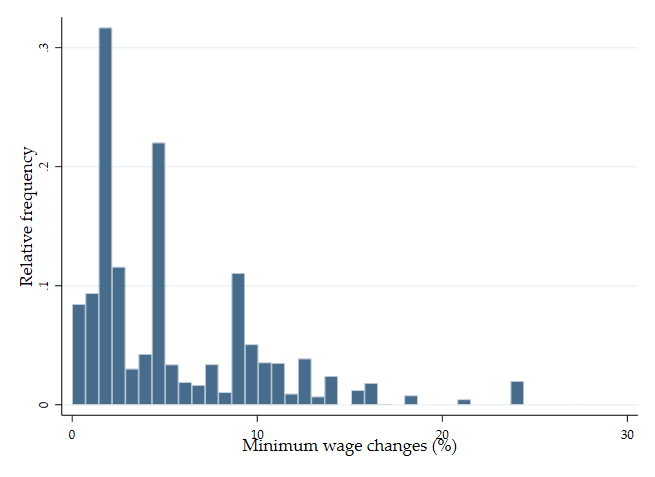
\includegraphics[width = \textwidth]
            {descriptive/estimation_samples/output/pct_ch_mw_dist}
    \end{subfigure}\\
    \begin{subfigure}{.7\textwidth}
        \caption{Timing}
        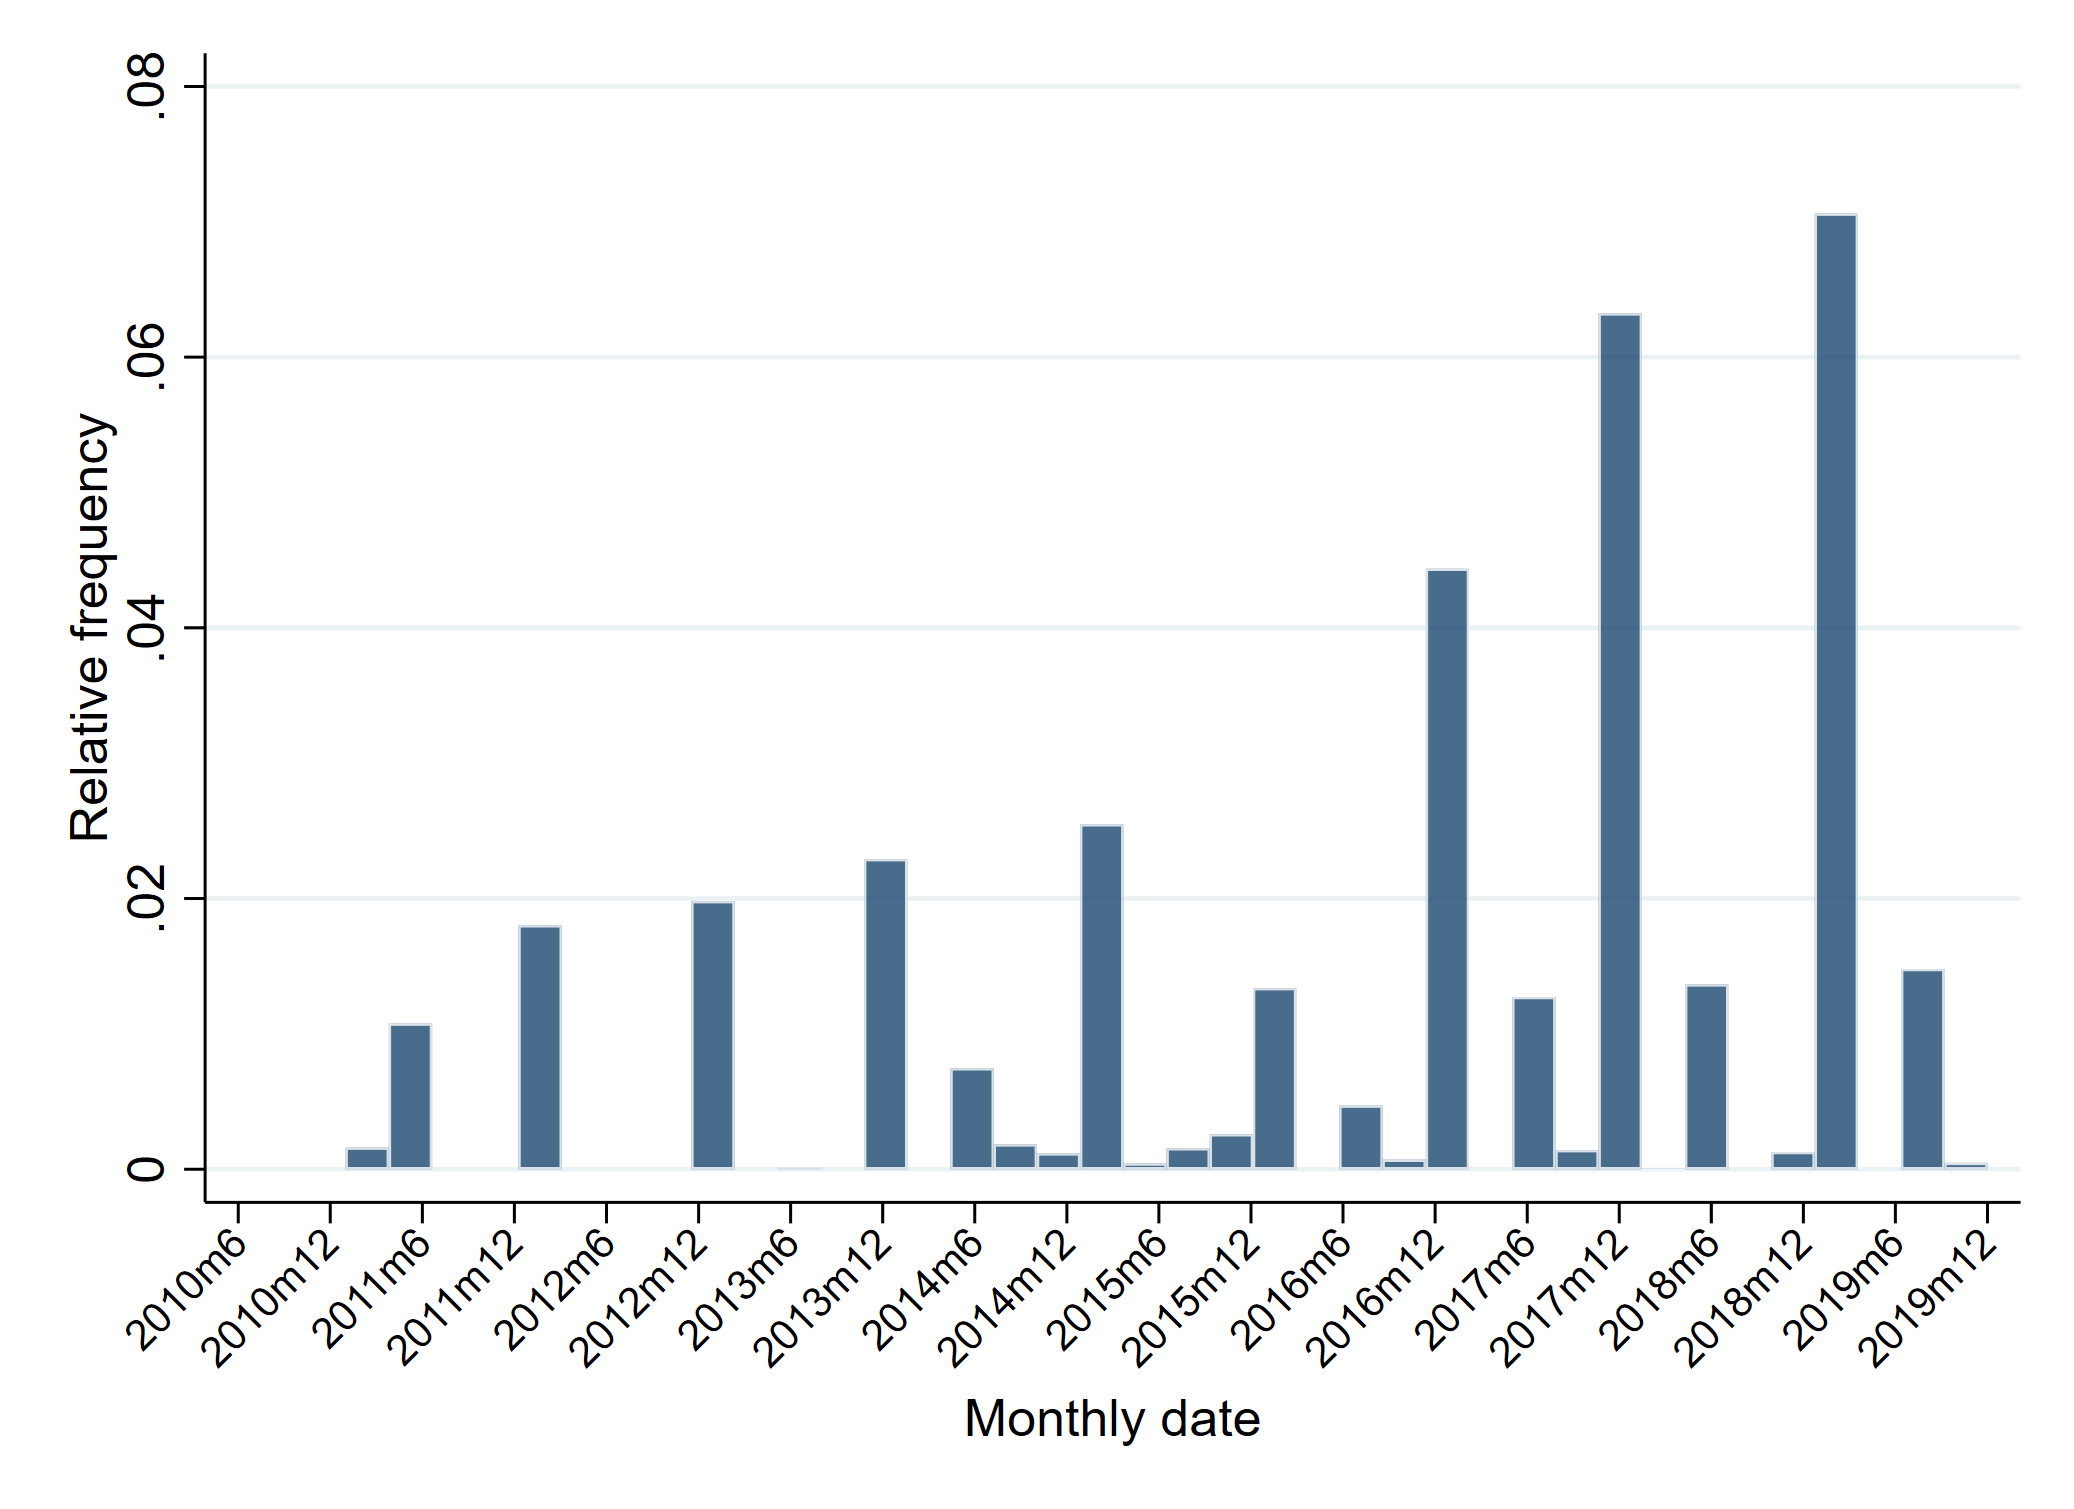
\includegraphics[width = \textwidth]
            {descriptive/estimation_samples/output/pct_ch_mw_date_dist}
    \end{subfigure}

    \begin{minipage}{.95\textwidth} \footnotesize
        \vspace{3mm}
        \textit{Notes:} The histograms show the distribution of positive MW changes 
        in the full sample of ZIP codes available in the Zillow data. Panel (a) reports 
        the intensity of the changes in percentage terms. Panel (b) plots the distribution 
        across time of such changes. 
    \end{minipage}
\end{figure}

\begin{figure}[h!]
	\centering
	\caption{Spatial Distribution of Minimum Wage Changes}
	\label{fig:mw_perc_changes_long_run}
	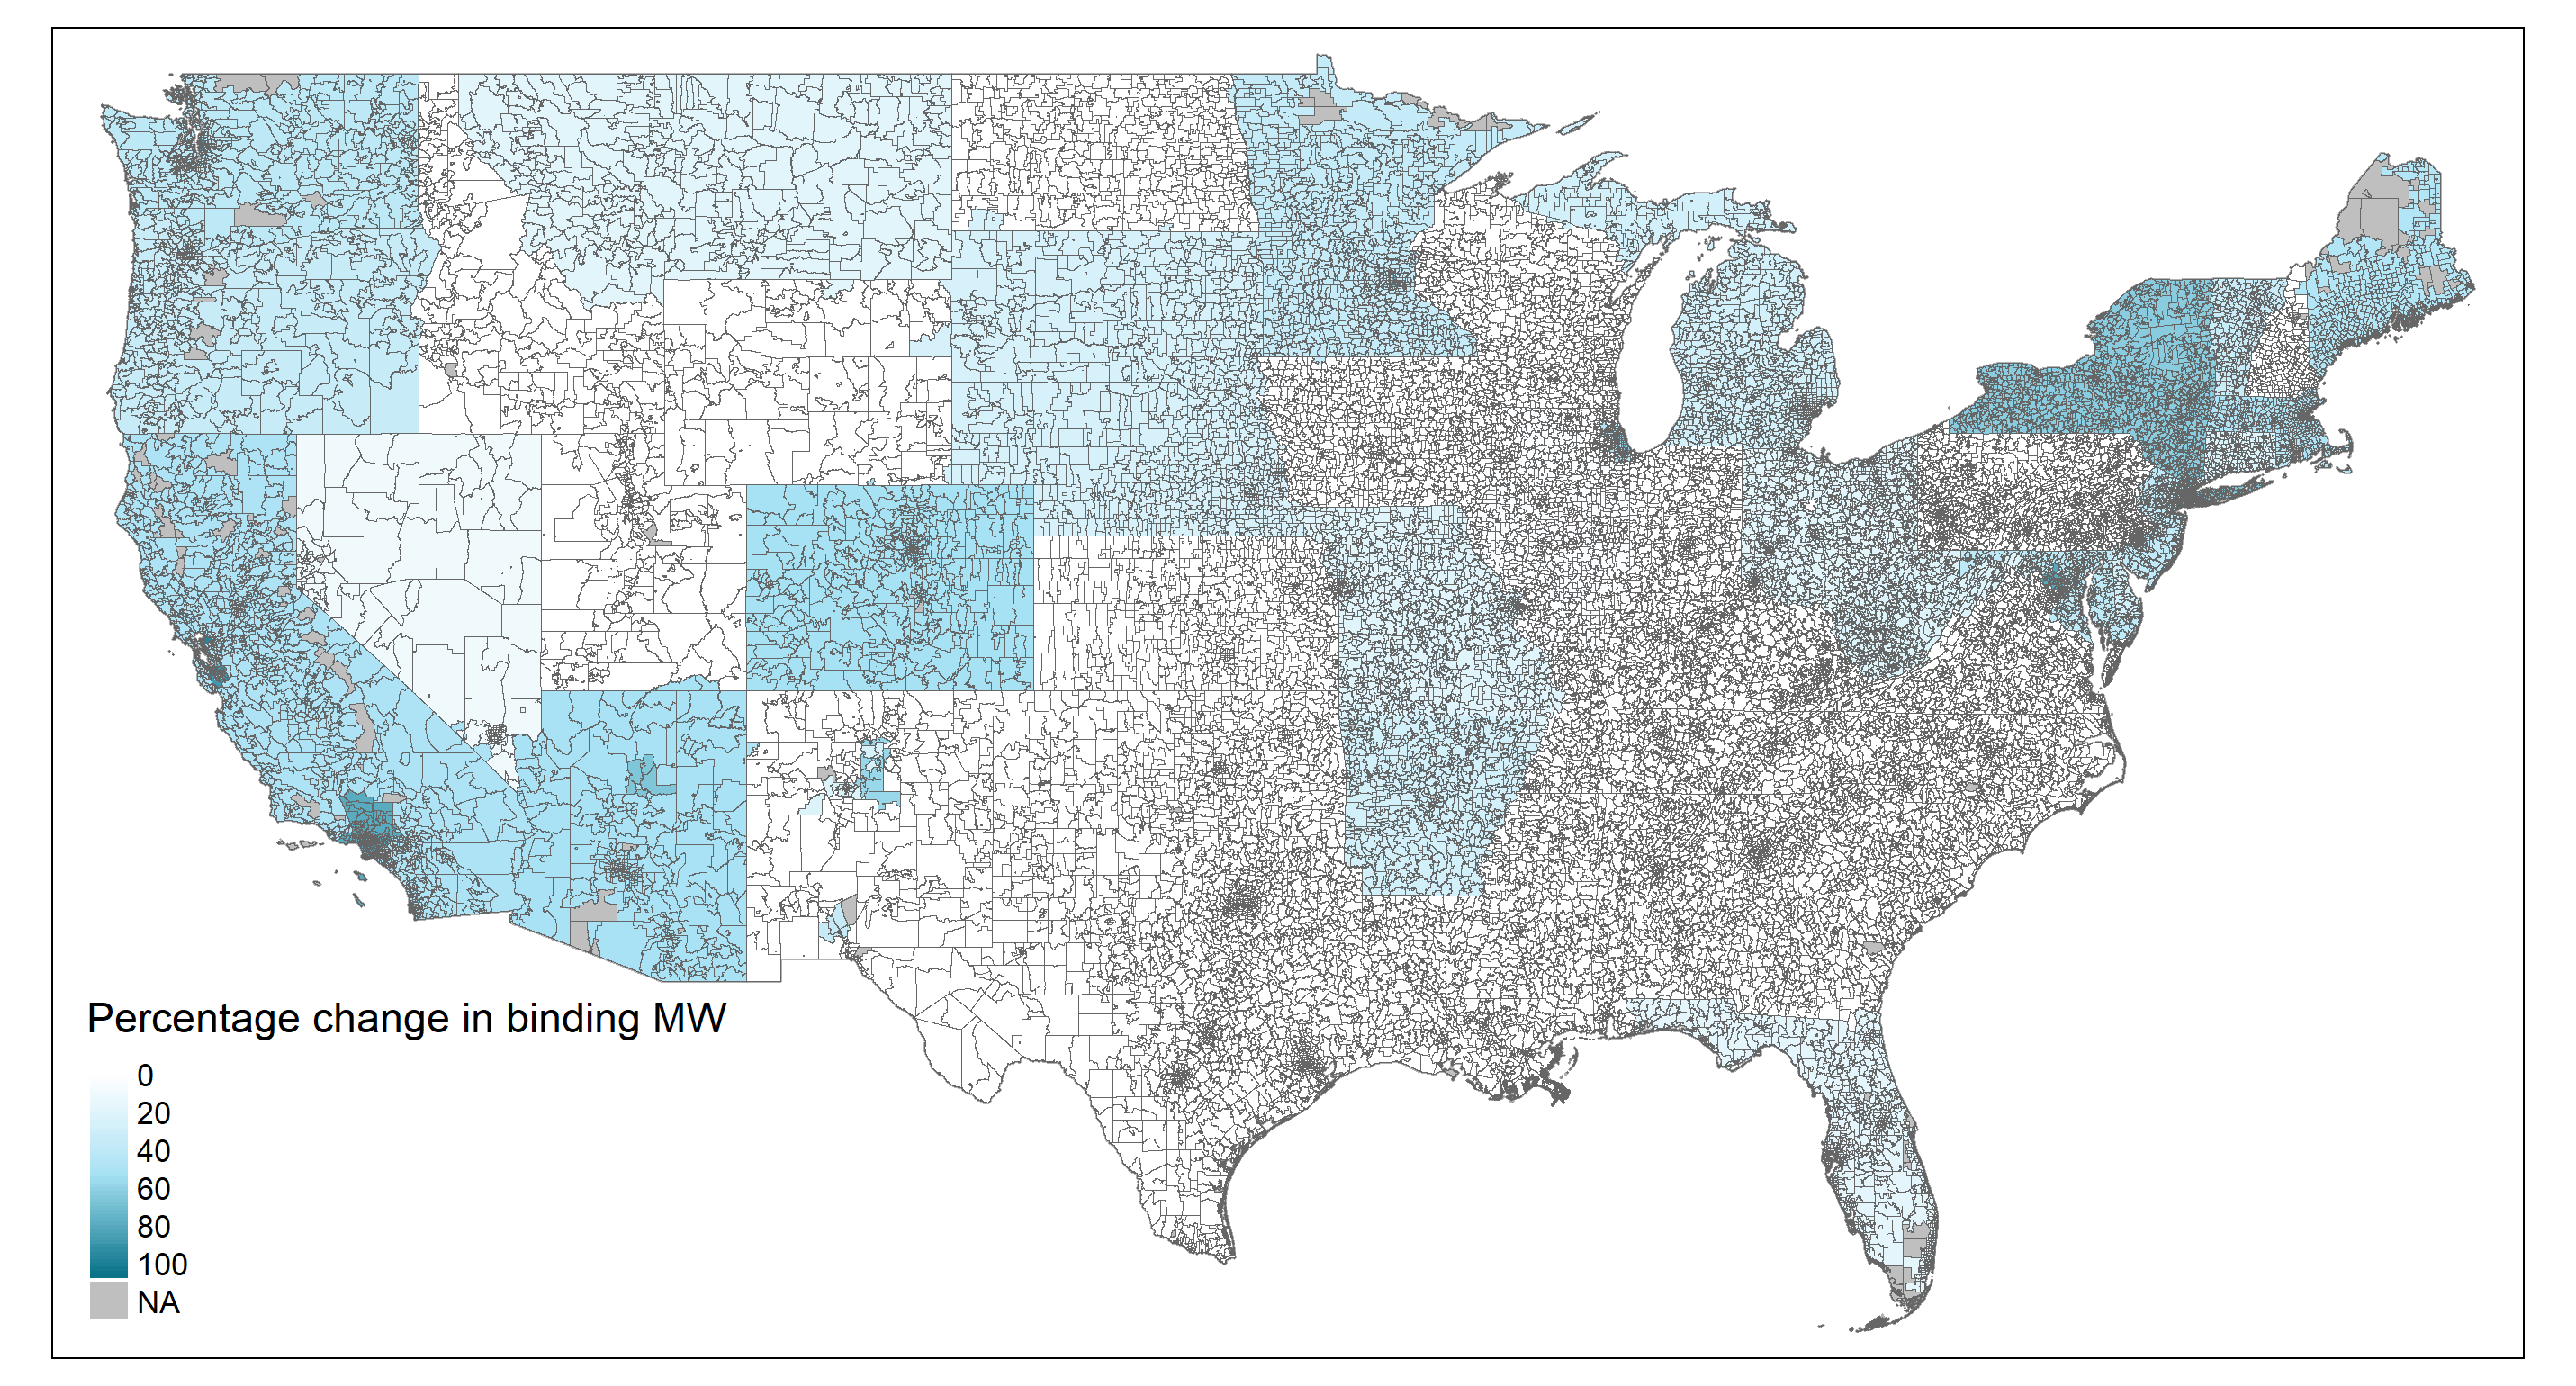
\includegraphics[width = \textwidth]
	    {../../analysis/maps_mw_long_run/output/USchange_perc_actual_mw.png}
	\begin{minipage}{.95\textwidth} \footnotesize
		\vspace{3mm}
		\textit{Notes:} This figure shows the percentage change in residence MW levels
		at each US ZIP code from January 2010 to December 2019.
	\end{minipage}
\end{figure}
